\documentclass{article}
\usepackage[english]{babel}
\usepackage{float}

\usepackage{graphicx}
\usepackage[colorlinks=true, allcolors=blue]{hyperref}

\usepackage[letterpaper,top=.5cm,bottom=2cm]{geometry}

\date{January 1, 2025}
\title{MidTerm Exam Paper}
\author{Terrence Jackson}

\begin{document}
\maketitle


\begin{abstract}
Is there a way to make embedded controls smarter? Controls systems are inherently rigid, based on requirements standards that implement code.  What if there was a way to have the Control System suggest better or more efficient ways to produce  a desired outcome.  What if the Control System user wasn't always correct in the input of the controls?
\end{abstract}

\section{Introduction}

By nature of the Control System architecture, the system should follow a rigid set of rules developed, architect,  and designed and documented by requirements set.  So what is expected to happen in a situation, should happen and react according to those set of standards. That is the basis of controls. 

Controls Systems have a basis where the system under control is managed in a way to perform a task and give certain outcome based on inputs that also include those controls.  Also, there is inherently a 'controller' which may be some user or set of users that react and input commands to that system.  Sometimes those controllers' inputs could be optimized.  

\section{Results}

The Chart \ref{fig:graph} below is a diagram showing how much of the inputs from outside users may affect the outcome of the Controls System given a set of inputs. These outcomes can vary greatly but may also be optimized in some cases to reduce the load and/or response time from the user. 

\begin{figure}[H]
\centering
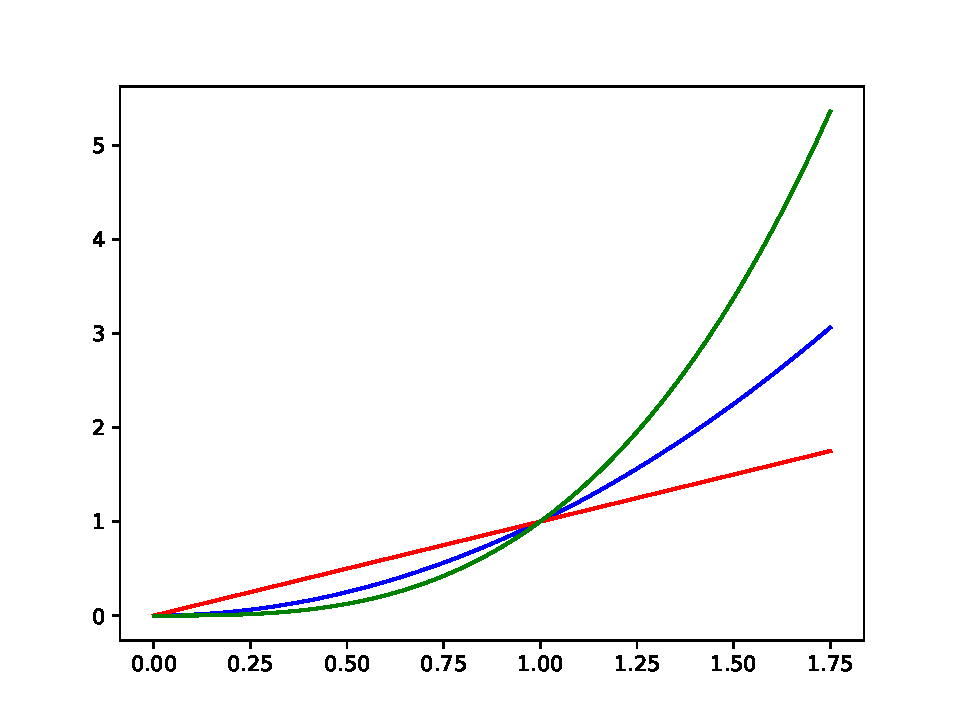
\includegraphics[width=0.65\linewidth]{Midterm_Jackson.pdf}
\caption{\label{fig:graph} Controls Systems Chart}
\end{figure}
    

\section{Conclusion}

Based on the outlined findings previously stated, it is within reason to conclude that Controls Systems can be improved in nominal/critical cases where time to react, outcomes desired, and other data factors may help to improve system efficiency and desired outcomes. 


\end{document}
